\documentclass[10pt,a4paper,titlepage]{article}
\usepackage[utf8]{inputenc}
\usepackage{amsmath}
\usepackage{amsfonts}
\usepackage{amssymb}
\usepackage{amsthm}
\usepackage{mathtools}
\usepackage[bottom]{footmisc}
\usepackage{pgfplots}
%\usepackage{parskip}

\usetikzlibrary{patterns}

\author{Felix Fritz}
\title{The Bondareva-Shapley Theorem}

\theoremstyle{plain}
\newtheorem{thm}{Theorem}[section] % reset theorem numbering for each chapter

\theoremstyle{definition}
\newtheorem{defn}[thm]{Definition} % definition numbers are dependent on theorem numbers
\newtheorem{exmp}[thm]{Example} % same for example numbers

\begin{document}
\maketitle

\tableofcontents
\pagebreak

\section{Cooperative Games and the Core}
 Before diving into the concept of balanced collections, balanced games and the Bondareva-Shapley Theorem, I want to establish a basic understanding of cooperative games, imputations and the core, mainly as it is described in Robert P. Gilles book \cite{gilles}, pp. 12--13, 18--20 and 29--35.

 First we introduce a formal definition of a cooperative game.

\begin{defn}
    The pair $(N, v)$ is a \textit{cooperative game} if $N$ is a finite player set and $v: 2^N \rightarrow \mathbb{R}$ is a characteristic function that assigns to every coalition $S \subseteq N$ an attainable payoff $v(S)$ such that $v(\emptyset) = 0$.
    
    For every player set $N$ we denote by $\mathcal{G}^N$ the class of all characteristic functions on $N$.
\end{defn}
Simply put, in a cooperative game we define collective payoff values for every possible coalition between players. A coalition without any players leads to a payoff of zero.

Suppose for a given cooperative game all players form a grand coalition generating a total payoff of $v(N)$. The ways in which we can distribute the collective wealth among each player can be described with a vector $x \in \mathbb{R}^N$, each element $x_i$ indicating what player $i \in N$ should receive.
If this vector fulfills the requirement needed for efficiency and individual rationality, we have an \textit{imputation}.

\begin{defn}
    An \textit{imputation} in the cooperative game $v \in \mathcal{G}^N$ is a vector $x = (x_1, ..., x_n) \in \mathbb{R}^N$ satisfying
    \[
        \begin{aligned}
            &x(N) = v(N) && \quad \text{(Efficiency)}\footnotemark\\
            &x_i \geq v(i)\text{ for every player } i \in N && \quad \text{(Individual rationality)\footnotemark}
        \end{aligned}
    \]
    \footnotetext[1]{For a given vector $x \in \mathbb{R}^N$ and a coalition $S \subseteq N$, $x(S)$ refers to the sum of elements $x_i$ for each player $i \in S$: $x(S) = \sum_{i \in S}x_i$}
    \footnotetext{Formally we would need curly braces around $i$ in the payoff function $v$ $\rightarrow v(\{i\})$. Because it is obvious that $v(i)$ indicates the payoff for a coalition containing the single player $i$, I will omit the braces.}
    The set of all vectors satisfying the efficiency and individual rationality constraint is the \textit{imputation set}.
    \begin{equation}\label{eq:imputation}
        I(N, v) \coloneqq \{x \in \mathbb{R}^N \mid x(N) = v(N),\quad x_i \geq v(i) \quad \forall i \in N\}
    \end{equation}
\end{defn}

With the imputation set, we ensure that each player at minimum receives a value they could have attained on their own.

If we take each possible coalition $S \subseteq N$ into account and verify that the value from an imputation $x(S) = \sum_{i \in S}x_i \geq v(S)$, we have an imputation that is \textit{coalitionally rational}.

\begin{defn}\label{def:core}
    A collection of coalitionally rational imputations is the \textit{core} of a cooperative game.
    \begin{equation}\label{eq:core}
        \mathcal{C}(N, v) \coloneqq \{x \in I(N, v) \mid x(S) \geq v(S)\quad \forall S \subseteq N\}
    \end{equation}
\end{defn}

 \section{Bondareva-Shapley Theorem}
 In the following chapter we will discuss the properties of cooperative games with a nonempty core and introduce the notion of balancedness, which leads us to the Bondareva-Shapley Theorem.

 \subsection{Nonempty Cores}
 For this section we want to focus on some of the properties that apply to cooperative games that have at least one imputation that is in the core set.

 From our definition of a core in \ref{def:core} it is easy to provide some examples of cooperative games that don't contain a core.

 \begin{exmp}
    Suppose we have game with $N = 2$ with the following payoffs: $v(\emptyset) = 0, v(1) = v(2) = 2, v(1, 2) = 3$.

    Determining if a core exists in such a situation may be trivial to solve, but with only two players this gives us the opportunity to plot a graph and visualize the solution concept.
    
    Because this is only a two-player game, there are no coalitions other than the grand coalition. This means that every imputation is automatically inside the core.

    For a vector $x \in \mathbb{R}^2$ to be an imputation, it has to be efficient and individually rational.

    \begin{tikzpicture}
        \begin{axis}[no marks,
            axis lines = left,
            xlabel = {Player 1},
            ylabel = {Player 2},
            xmin = 0, xmax = 3.5,
            ymin = 0, ymax = 3.5,
            xtick={1,2,3},
        ]
            

            %what player 1 wants
            \filldraw [draw=none,pattern=north east lines] (0, 0) rectangle (400, 400);
            \addplot [blue, thick]{2};
            % \addplot [blue, thick] coordinates {(2,0)(2,3.5)};
            

            % %efficient payoff function
            % \addplot [color=red, thick]{-x+3};
        \end{axis}
    \end{tikzpicture}
 \end{exmp}

 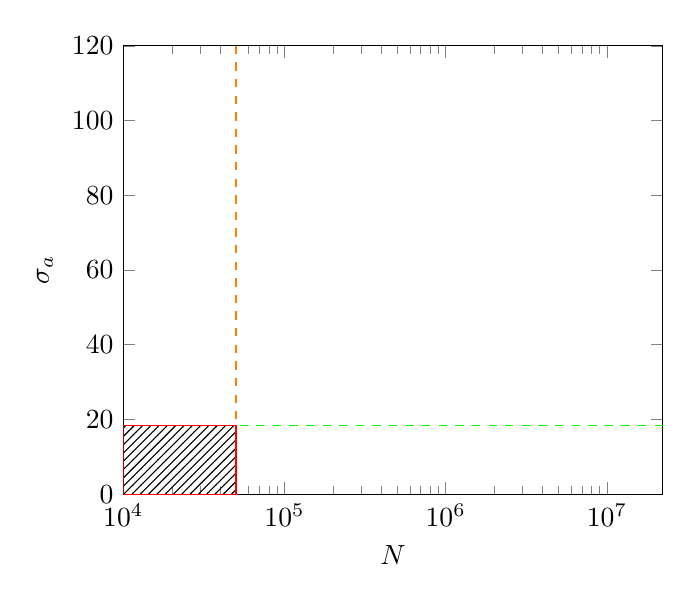
\begin{tikzpicture}
    \begin{semilogxaxis}
      [
          enlarge x limits=false,
          no marks,
          grid=none,
          xmin=1e4, xmax=22260785,
          ymin=0, ymax=120,
          ylabel={$\sigma_{a}$},
          xlabel={$N$},
          samples=400 
       ]
         \begin{scope}[green] 
           \draw[orange,dashed] ({axis cs:50045,0}|-{rel axis cs:0,1}) -- ({axis cs:50045,0}|-{rel axis cs:0,0});
           \draw[dashed,green] ({rel axis cs:1,0}|-{axis cs:0,18.385735235}) -- ({rel axis cs:0,0}|-{axis cs:0,18.385735235});
           \filldraw [draw=red,pattern=north east lines] (rel axis cs:0,0) rectangle (axis cs:50045,18.385735235);
         \end{scope}
    \end{semilogxaxis}
  \end{tikzpicture}
 

 \subsection{Balanced Games}

 \subsection{The Bondareva-Shapley Theorem}

 \section{Market Games with nonempty cores}
 Market games can be proven to have a non-empty core using the Bondareva-Shapley Theorem. We will take a closer look on how this can be achieved in the third chapter.

 \section{Proving the Theorem using Linear Programming}
 Finally, we will show that the Bondareva-Theorem holds true with a prove using the Duality Problem in Linear Programming.
 
\pagebreak
 
\bibliographystyle{unsrt}
\bibliography{references}
\end{document}